% ------------------------------------------------------------------------
% ------------------------------------------------------------------------
% Modelo UFSC para Trabalhos Academicos (tese de doutorado, dissertação de
% mestrado) utilizando a classe abntex2
%
% Autor: Alisson Lopes Furlani
% 	Modificações:
%	- 27/08/2019: Alisson L. Furlani, add pacote 'glossaries' para listas
% - 30/10/2019: Alisson L. Furlani, adjusted some spacing errors and changed math fonts
% - 17/01/2019: Alisson L. Furlani, updated certification page
% - 03/03/2020: Luiz F. P. Droubi, change file to be used as a template with R.

% eu (francisco) fiz adaptações pra tese USP

% ------------------------------------------------------------------------
% ------------------------------------------------------------------------

\documentclass[
	% -- opções da classe memoir --
	12pt,				% tamanho da fonte
	%openright,			% capítulos começam em pág ímpar (insere página vazia caso preciso)
	oneside,			% para impressão no anverso. Oposto a twoside
	a4paper,			% tamanho do papel.
	% -- opções da classe abntex2 --
	chapter=TITLE,		% títulos de capítulos convertidos em letras maiúsculas
	section=TITLE,		% títulos de seções convertidos em letras maiúsculas
	%subsection=TITLE,	% títulos de subseções convertidos em letras maiúsculas
	%subsubsection=TITLE,% títulos de subsubseções convertidos em letras maiúsculas
	% -- opções do pacote babel --
	brazil,			% idioma adicional para hifenização
	%french,				% idioma adicional para hifenização
	%spanish,			% idioma adicional para hifenização
	english				% o último idioma é o principal do documento
	]{abntex2}

\usepackage{setup/ufscthesisA4-alf}

\addbibresource{bib/ch1.bib}
\addbibresource{bib/references.bib}
\addbibresource{bib/pkgs.bib}

\usepackage[table]{xcolor}
\let\newfloat\undefined
\usepackage{floatrow}
\floatsetup[table]{capposition=top}
\floatsetup[figure]{capposition=bottom} % regula posicao da legenda!

\newcommand{\pkg}[1]{{\normalfont\fontseries{b}\selectfont #1}}
\let\proglang=\textsf
\let\code=\texttt


\newcommand{\bcenter}{\begin{center}}
\newcommand{\ecenter}{\end{center}}

\newcommand{\bapendices}{\begin{apendicesenv}}
\newcommand{\eapendices}{\end{apendicesenv}}

\newcommand{\banexos}{\begin{anexosenv}}
\newcommand{\eanexos}{\end{anexosenv}}

%################################

% alteracao de template pra funcionar bib!!

%################################

%opcao 1:
% \newlength{\cslhangindent}
%\setlength{\cslhangindent}{1.5em}
%\newenvironment{CSLReferences}%
%{\setlength{\parindent}{0pt}%
%\everypar{\setlength{\hangindent}{\cslhangindent}}\ignorespaces}%
%{\par}

% opcao 2

 

% ---
% Filtering and Mapping Bibliographies
% ---
\DeclareSourcemap{
	\maps[datatype=bibtex]{
		% remove fields that are always useless
		\map{
			\step[fieldset=abstract, null]
			\step[fieldset=pagetotal, null]
		}
		% remove URLs for types that are primarily printed
%		\map{
%			\pernottype{software}
%			\pernottype{online}
%			\pernottype{report}
%			\pernottype{techreport}
%			\pernottype{standard}
%			\pernottype{manual}
%			\pernottype{misc}
%			\step[fieldset=url, null]
%			\step[fieldset=urldate, null]
%		}
		\map{
			\pertype{inproceedings}
			% remove mostly redundant conference information
			\step[fieldset=venue, null]
			\step[fieldset=eventdate, null]
			\step[fieldset=eventtitle, null]
			% do not show ISBN for proceedings
			\step[fieldset=isbn, null]
			% Citavi bug
			\step[fieldset=volume, null]
		}
	}
}
% ---

% ---
% Informações de dados para CAPA e FOLHA DE ROSTO
% ---
% FIXME Substituir 'Nome completo do autor' pelo seu nome.
\autor{FRANCISCO D'ALBERTAS GOMES DE CARVALHO}
% FIXME Substituir 'Título do trabalho' pelo título da trabalho.
\titulo{TÍTULO}
% FIXME Substituir 'Subtítulo (se houver)' pelo subtítulo da trabalho.
% Caso não tenha substítulo, comente a linha a seguir.
  \subtitulo{SUBTÍTULO}
% FIXME Substituir 'XXXXXX' pelo nome do seu
% orientador.
\orientador{Jean Paul Meztger}
% FIXME Se for orientado por uma mulher, comente a linha acima e descomente a linha a seguir.
% \orientador[Orientadora]{Nome da orientadora, Dra.}
% FIXME Substituir 'XXXXXX' pelo nome do seu
% coorientador. Caso não tenha coorientador, comente a linha a seguir.
% FIXME Se for coorientado por uma mulher, comente a linha acima e descomente a linha a seguir.
% \coorientador[Coorientadora]{XXXXXX, Dra.}
% FIXME Substituir '[ano]' pelo ano (ano) em que seu trabalho foi defendido.
\ano{2022}
% FIXME Substituir '[dia] de [mês] de [ano]' pela data em que ocorreu sua defesa.
\data{xx de Fevereiro de 2022}
% FIXME Substituir 'Local' pela cidade em que ocorreu sua defesa.
\local{São Paulo}
\instituicaosigla{USP}
\instituicao{Universidade de São Paulo}
% FIXME Substituir 'Dissertação/Tese' pelo tipo de trabalho (Tese, Dissertação).
\tipotrabalho{tese}
% FIXME Substituir '[mestre/doutor] em XXXXXX' pela grau adequado.
\formacao{Doutor em Ecologia}
% FIXME Substituir '[mestrado/doutorado]' pelo nivel adequado.
\nivel{doutorado}
% FIXME Substituir 'Programa de Pós-Graduação em XXXXXX' pela curso adequado.
\programa{Programa de Pós-Graduação em Ecologia}
% FIXME Substituir 'Campus XXXXXX ou Centro de XXXXXX' pelo campus ou centro adequado.
\centro{Instituto de Biosciências}
\preambulo
{%
\imprimirtipotrabalho~submetida~ao~\imprimirprograma~da~\imprimirinstituicao~para~a~obtenção~do~título~de~\imprimirformacao.
}
% ---

% ---
% Configurações de aparência do PDF final
% ---
% alterando o aspecto da cor azul
\definecolor{blue}{RGB}{41,5,195}
% informações do PDF
\makeatletter
\hypersetup{
     	%pagebackref=true,
		pdftitle={\@title},
		pdfauthor={\@author},
    	pdfsubject={\imprimirpreambulo},
	    pdfcreator={LaTeX with abnTeX2},
		pdfkeywords={ufsc, latex, abntex2},
		colorlinks=true,       		% false: boxed links; true: colored links
    	linkcolor=black,%blue,          	% color of internal links
    	citecolor=black,%blue,        		% color of links to bibliography
    	filecolor=black,%magenta,      		% color of file links
		urlcolor=black,%blue,
		bookmarksdepth=4
}
\makeatother
% ---

% ---
% compila a lista de abreviaturas e siglas e a lista de símbolos
% ---

% Declaração das siglas
%\siglalista{ABNT}{Associação Brasileira de Normas Técnicas}
\siglalista{Bacen}{Banco Central do Brasil}


% Declaração dos simbolos
%\simbololista{C}{\ensuremath{C}}{Circunferência de um círculo}
\simbololista{pi}{\ensuremath{\pi}}{Número pi}
\simbololista{r}{\ensuremath{r}}{Raio de um círculo}
\simbololista{A}{\ensuremath{A}}{Área de um círculo}


% compila a lista de abreviaturas e siglas e a lista de símbolos
%\makenoidxglossaries

% ---

% ---
% compila o indice
% ---
\makeindex
% ---

% ----
% Início do documento
% ----
\begin{document}

% Seleciona o idioma do documento (conforme pacotes do babel)
%\selectlanguage{english}
\selectlanguage{brazil}

% Retira espaço extra obsoleto entre as frases.
\frenchspacing

% Espaçamento 1.5 entre linhas
\OnehalfSpacing

% Corrige justificação
%\sloppy

% ----------------------------------------------------------
% ELEMENTOS PRÉ-TEXTUAIS
% ----------------------------------------------------------
% \pretextual %a macro \pretextual é acionado automaticamente no início de \begin{document}
% ---
% Capa, folha de rosto, ficha bibliografica, errata, folha de apróvação
% Dedicatória, agradecimentos, epígrafe, resumos, listas
% ---
% ---
% Capa
% ---
\imprimircapa
% ---

% ---
% Folha de rosto
% (o * indica que haverá a ficha bibliográfica)
% ---
\imprimirfolhaderosto*
% ---

% ---
% Inserir a ficha bibliografica
% ---
% http://ficha.bu.ufsc.br/
\begin{fichacatalografica}
	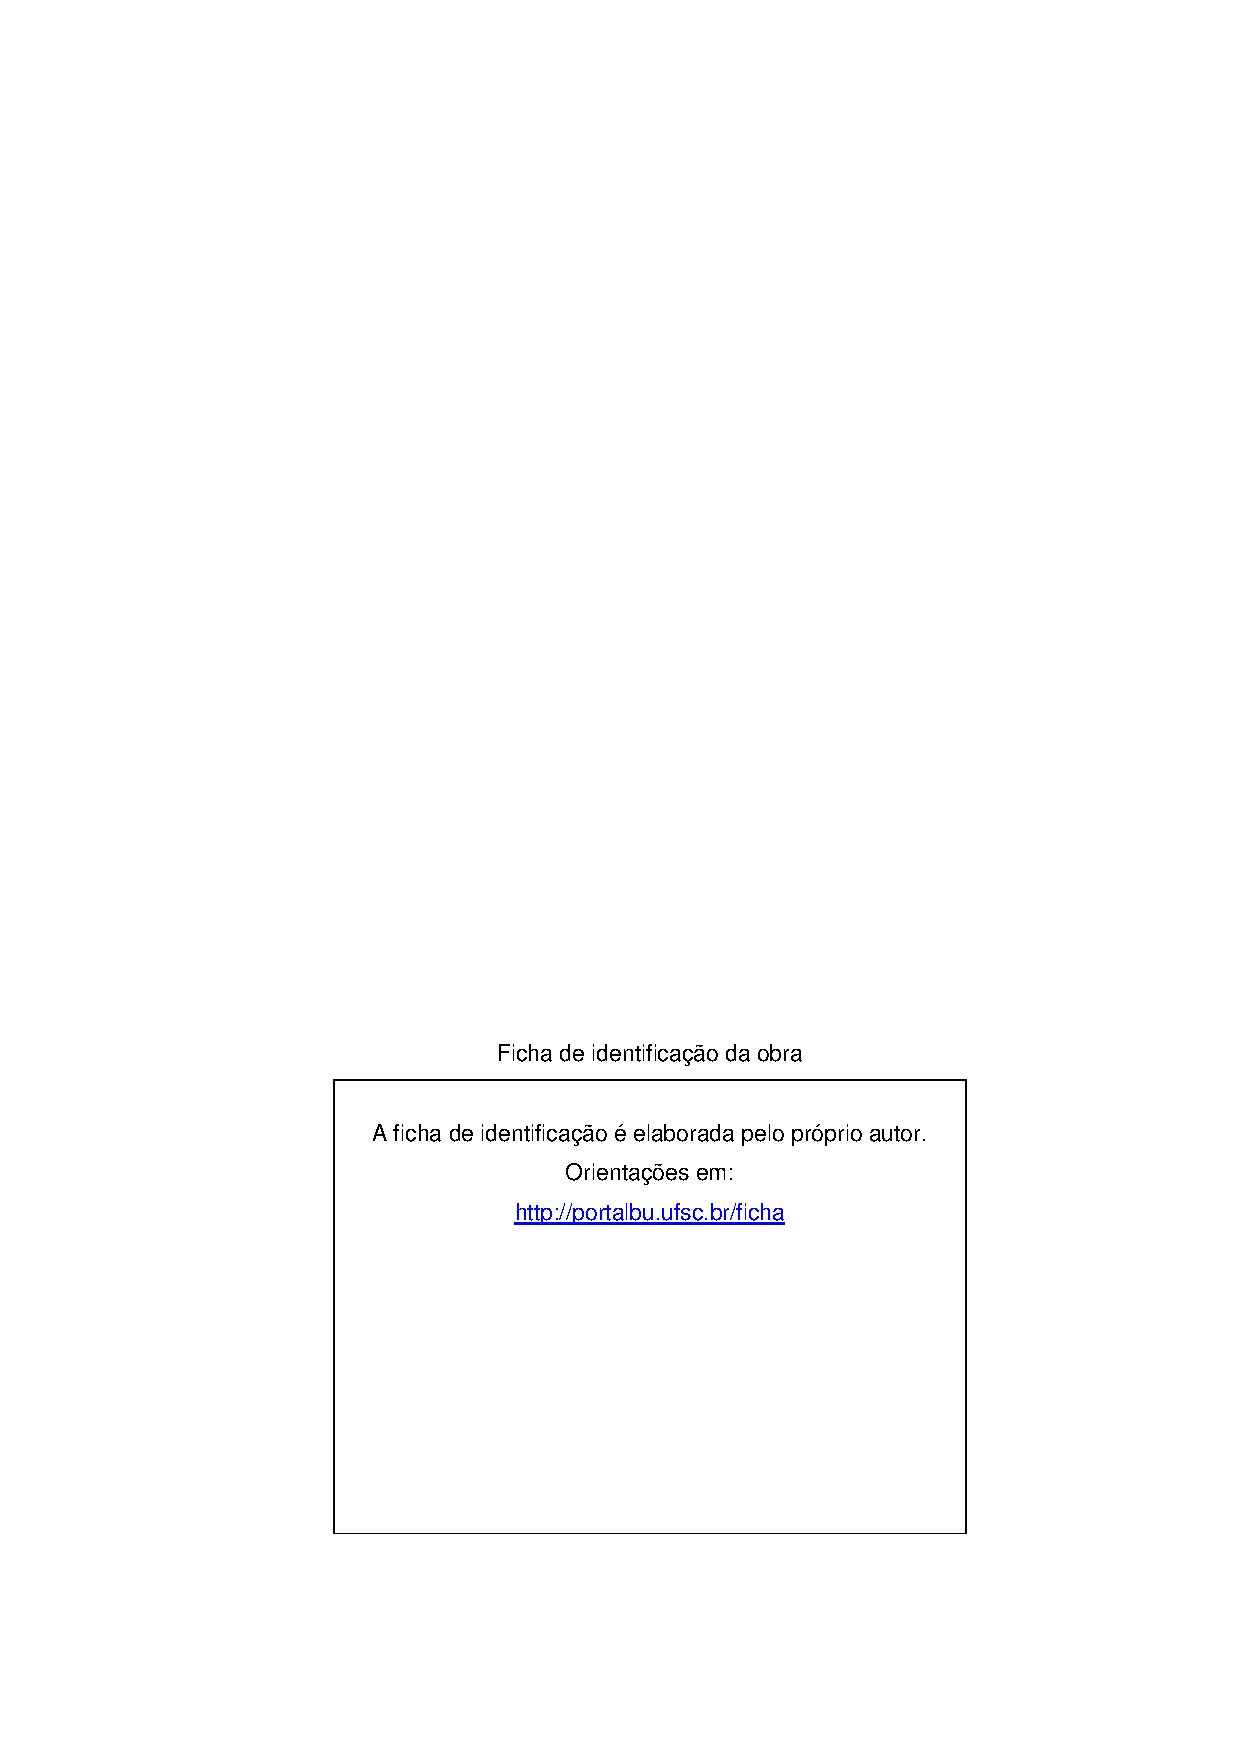
\includepdf{Ficha_Catalografica.pdf}
\end{fichacatalografica}
% ---

% ------------------------------------------------
% Inserir folha de aprovação (eu exclui)!
% ------------------------------------------------
%\begin{folhadeaprovacao}
%	\OnehalfSpacing
%	\centering
%	\imprimirautor\\%
%	\vspace*{10pt}		
%	\textbf{\imprimirtitulo}%
%	\ifnotempty{\imprimirsubtitulo}{:~\imprimirsubtitulo}\\%
	%		\vspace*{31.5pt}%3\baselineskip
%	\vspace*{\baselineskip}
%	%\begin{minipage}{\textwidth}
%	O presente trabalho em nível de \imprimirnivel~foi avaliado e aprovado por banca examinadora composta pelos seguintes membros:\\
%	%\end{minipage}%
%	\vspace*{\baselineskip}
  %  %Prof. Examinador 1, Dr.\\
  %Universidade Federal de Santa Catarina - UFSC\\
  %\vspace*{\baselineskip}
 %   %Prof. Examinador 2eh, Dr.\\
  %Fédération Internationale des Géomètres - FIG\\
  %\vspace*{\baselineskip}
 %   
%	\vspace*{2\baselineskip}
%	\begin{minipage}{\textwidth}
%		Certificamos que esta é a \textbf{versão original e final} do trabalho de conclusão que foi julgado adequado para obtenção do título de \imprimirformacao.\\
%	\end{minipage}
%	%    \vspace{-0.7cm}
%	\vspace*{\fill}
%	\assinatura{\OnehalfSpacing Beltrano da Silva \\ Coordenação do Programa de Pós-Graduação}
%	\vspace*{\fill}
%	\assinatura{\OnehalfSpacing\imprimirorientador \\ \imprimirorientadorRotulo}
	%	\ifnotempty{\imprimircoorientador}{
	%	\assinatura{\imprimircoorientador \\ \imprimircoorientadorRotulo \\
	%		\imprimirinstituicao~--~\imprimirinstituicaosigla}
	%	}
	% \newpage
%	\vspace*{\fill}
%	\imprimirlocal, \imprimirano.
%\end{folhadeaprovacao}
% ---

% ---
% Dedicatória
% ---
\begin{dedicatoria}
	\vspace*{\fill}
	\noindent
	\begin{adjustwidth*}{}{5.5cm} 
		\raggedleft       
		elaborar dedicatória
	\end{adjustwidth*}
\end{dedicatoria}
% ---

% ---
% Agradecimentos
% ---
\begin{agradecimentos}
	Gostaria de agradecer sinceramente a todos os que colaboraram à execução\\
 deste trabalho.\\
 Aos colegas da UFSC.\\
 Aos professores do PPGTG.\\
 Em especial ao meu orientador, pela paciência.\\
 E a minha querida esposa pela compreensão.
\end{agradecimentos}
% ---

% ---
% Epígrafe
% ---
\begin{epigrafe}
	\vspace*{\fill}
	\begin{flushright}
		\textit{``Colocar epígrafe, talvez eliane brum''\\
(citação da obra)}
	\end{flushright}
\end{epigrafe}
% ---

% ---
% RESUMOS
% ---

% resumo em português
\setlength{\absparsep}{18pt} % ajusta o espaçamento dos parágrafos do resumo
\begin{resumo}
	\SingleSpacing
  Escrever o resumo e checar por erros com acentuação! 
  
  \textbf{Palavras-chave}: 
    Palavra-chave 1.
    Palavra-chave 2.
  \end{resumo}
% resumo em inglês
\begin{resumo}[Abstract]
	\SingleSpacing
	\begin{otherlanguage*}{english}
		Resumo geral em inglês
		
		\textbf{Keywords}:
	      Keyword 1.
        Keyword 2.
    	\end{otherlanguage*}
\end{resumo}
%% resumo em francês 
%\begin{resumo}[Résumé]
% \begin{otherlanguage*}{french}
%    Il s'agit d'un résumé en français.
% 
%   \textbf{Mots-clés}: latex. abntex. publication de textes.
% \end{otherlanguage*}
%\end{resumo}
%
%% resumo em espanhol
%\begin{resumo}[Resumen]
% \begin{otherlanguage*}{spanish}
%   Este es el resumen en español.
%  
%   \textbf{Palabras clave}: latex. abntex. publicación de textos.
% \end{otherlanguage*}
%\end{resumo}
%% ---

{%hidelinks
	\hypersetup{hidelinks}
	% ---
	% inserir lista de ilustrações
	% ---
	\pdfbookmark[0]{\listfigurename}{lof}
	\listoffigures*
	\cleardoublepage
	% ---
	
	% ---
	% inserir lista de quadros
	% ---
	%\pdfbookmark[0]{\listofquadrosname}{loq}
	%\listofquadros*
	%\cleardoublepage
	% ---
	
	% ---
	% inserir lista de tabelas
	% ---
	\pdfbookmark[0]{\listtablename}{lot}
	\listoftables*
	\cleardoublepage
	% ---
	
	% ---
	% inserir lista de abreviaturas e siglas (devem ser declarados no preambulo)
	% ---
	%\imprimirlistadesiglas
	% ---
	
	% ---
	% inserir lista de símbolos (devem ser declarados no preambulo)
	% ---
	%\imprimirlistadesimbolos
	% ---
	
	% ---
	% inserir o sumario
	% ---
	\pdfbookmark[0]{\contentsname}{toc}
	\tableofcontents*
	\cleardoublepage
	
}%hidelinks
% ---

% ---

% ----------------------------------------------------------
% ELEMENTOS TEXTUAIS
% ----------------------------------------------------------
\textual

\renewcommand{\figurename}{Figure}
\renewcommand{\tablename}{Table}

\hypertarget{introduuxe7uxe3o}{%
\chapter{Introdução}\label{introduuxe7uxe3o}}

\hypertarget{objetivos}{%
\section{Objetivos}\label{objetivos}}

Nas seções abaixo estão descritos o objetivo geral e os objetivos
específicos.

\hypertarget{objetivo-geral}{%
\subsection{Objetivo Geral}\label{objetivo-geral}}

Descrição

\hypertarget{objetivos-especuxedficos}{%
\subsection{Objetivos Específicos}\label{objetivos-especuxedficos}}

Descrição\ldots{}

\hypertarget{private-reserves-suffers-from-the-same-location-biases-of-public-protected-areas}{%
\chapter{Private reserves suffers from the same location biases of public protected areas}\label{private-reserves-suffers-from-the-same-location-biases-of-public-protected-areas}}

\(~\)
\begin{flushleft}

Francisco d’Albertas, Adrian González-Chaves, Clarice Borges-Matosa, Vitor
Zago de Almeida Paciello, Martine Maron, Jean Paul Metzger    

\end{flushleft}
\(~\)
\(~\)
\begin{flushleft}

This chapter was published as:

\end{flushleft}
\begin{flushleft}

d’ALBERTAS, F. et al. Private reserves suffer from the same location biases of public protected areas. Biological Conservation, v. 261, p. 109283, 1 set. 2021. 10.1016/j.biocon.2021.109283

\end{flushleft}
\(~\)
\(~\)

\hypertarget{abstract}{%
\section{Abstract}\label{abstract}}

Setting aside areas for conservation on private properties is an essential component of the response to the biodiversity crisis. Often this is voluntary, but in Brazil, landowners are required to set aside between 20\%-80\% of their property for native vegetation, in what are called Legal Reserves. If degraded, they need to be restored. Alternatively, landowners can compensate for a Legal Reserve deficit on their own property by purchasing surplus credits from another property. Each landowner can define the location and spatial arrangement of their Legal Reserves within their properties, affecting the ability of the reserves to maintain biodiversity and provide ecosystem services. To identify the drivers determining the amount and location of those Legal Reserves, we accessed data for 3,622 rural properties in southeastern Brazil. We found that the likelihood of a landowner setting aside part of their farm as Legal Reserve (avoiding off-farm compensation) increased with farm size and extent of native vegetation cover, particularly where this vegetation is along rivers and steep slopes, where conserving vegetation is also mandated in what are called Areas of Permanent Protection. Properties with these characteristics located in areas of higher transportation costs and lower agricultural suitability were more likely to have the full Legal Reserve requirement within their areas. Within properties, the location of Legal Reserves was mostly in areas of the property with low agricultural suitability, high transportation cost and close to Areas of Permanent Protection. These two results suggest landowners' decisions are made to maximize property income and to reduce restoration costs. Conservation on private land in Brazil thus follows similar patterns to public protected areas, being mostly located on marginal land for agriculture. These areas do not necessarily provide the greatest potential biodiversity and ecosystem services benefits, suggesting that specific government interventions may be needed to encourage landowners to set aside native vegetation in ways that maximise conservation and ecosystem service outcomes.
\begin{flushleft}

\textbf{Keywords}: private-land conservation,land-regulation,environmental policy, Forest Code,
  Natural Vegetation Protection Law, Atlantic Forest

\end{flushleft}
\hypertarget{introduction}{%
\section{Introduction}\label{introduction}}

One of the main policies in response to the biodiversity crisis \autocite{cardinale_biodiversity_2012,ipbes_unedited_2019} is the creation of new protected areas worldwide \autocite{unep-wcmc_protected_2018}. However, the location of public protected areas show a strong bias towards lands with high elevation, steeper slopes, low agricultural productivity, and low human density, not always considering biodiversity hotspots or ecological representativeness \autocite{venter_bias_2018,watson_performance_2014}. Thus, there is a clear need to reduce these biases.

One way to reduce bias is to increase protected areas on private land \autocite{cortes_capano_emergence_2019,drescher_practice_2018}. Agriculture cover \textgreater{} 30\% of the Earth's ice-free surface \autocite{ellis_anthropogenic_2010}, mostly on private property. In turn, private properties shelter vasts amounts of native vegetation, for instance, 56\% of the United States forests \autocite{sass_forest_2017}, 28\% of Europe's forests \autocite{pulla_mapping_2013} and 53\% of the native vegetation in Brazil \autocite{freitas_who_2017}. Protecting or enhancing natural vegetation on private properties also has benefits to private landholders beyond conservation itself. Native vegetation within farms can help increase agricultural production through the provision of ecosystem services \autocite{dainese_global_2019}. Natural pest control and pollination provided by native vegetation \autocite{boesing_effects_2017,potts_safeguarding_2016,rand_spillover_2006} make economic contributions between US\$ 10-1500 per hectare globally \autocite{lautenbach_spatial_2012,naranjo_economic_2015,pimentel_economic_1997}.

Some countries are implementing policies to set aside private areas for conservation in voluntary or mandatory schemes \autocite{garibaldi_positive_2019}. Brazil, in particular, has an environmental regulation, the Native Vegetation Protection Law (Federal Law 12.651/2012), which establishes that all rural properties must have natural vegetation set aside as mandatory Areas of Permanent Protection (APP; sensitive areas such as riparian vegetation, hilltops, and steep slopes) and Legal Reserves. Legal Reserves should cover from 20\% to 80\% of the total property area, depending on the Country's biome and physiognomy, and can include APP. Farmers that do not have the full area of Legal Reserves vegetated must restore it, or opt for a compensation scheme outside their property (for example, trading with landowners with Legal Reserves surplus). The latter strategy aims to allow properties with high opportunity costs to conserve or restore less valuable areas outside their limits \autocite{may_environmental_2015}. Legal Reserves are designed for the sustainable management of ecosystem services provided by natural vegetation and can combine native and non-native species (up to 50\% of Legal Reserves area). They are of vital importance for biodiversity protection, water and energy security, climate regulation, and ecosystem service provision \autocite{metzger_why_2019}.

At present, Legal Reserves cover 167 million ha \autocite{metzger_why_2019}, representing nearly half of the remaining native vegetation areas in Brazil \autocite{soares-filho_cracking_2014}, highlighting the importance of their maintenance. The proportion of vegetation in Legal Reserves is highest for the Atlantic Forest biome (70\% of remnant vegetation), where most of the Brazilian population lives \autocite{rezende_hotspot_2018}. Nevertheless, to achieve the objectives of Legal Reserves, their location should be adequately planned to support species survival in fragmented landscape \autocite{fahrig_ecological_2017,tambosi_framework_2014} while favoring ecosystem services that can increase agricultural productivity \autocite{boesing_effects_2017,garibaldi_stability_2011}.

To enforce the implementation of the Native Vegetation Protection Law, in 2012 the Brazilian Government created a self-declaratory public-access database, named CAR (Portuguese acronym for environmental rural register), in which each landowner delimits the size and location of their Legal Reserves. This extensive CAR database, gathering more than 5.6 million properties and nearly 550 million ha of land (in July 2020), offers a unique opportunity to evaluate landowner's management choices in response to a land-regulation policy.

Here we use CAR data to shed light on which drivers affect farmer's decisions about the amount and spatial location of Legal Reserves within their properties and consider the implications of their choices for biodiversity conservation and ecosystem services provision. We address two important questions: (1) which drivers predict the proportion of Legal Reserves the landowners declare inside their properties versus outside their land? (2) For landowners that decided to allocate Legal Reserves inside their properties, which drivers can predict where those Legal Reserves are located?
Following the pattern already described for public protected areas (Venter et al., 2018; Watson et al., 2014), we expected that land management decisions concerning Legal Reserves are made to maximize farm income. Farms located in marginal areas for agriculture production or less profitable were thus expected to set aside larger proportions of Legal Reserves inside their properties. We also expected that larger properties will declare higher proportions of Legal Reserves on-property. Considering the same reasoning, we also expected landowners will tend to locate their Legal Reserves within marginal lands. Additionally, we evaluated whether farmers are choosing to allocate Legal Reserves near existing native vegetation patches, which would increase patch size and could contribute to biodiversity conservation and ecosystem services provision.

\hypertarget{methods}{%
\section{Methods}\label{methods}}

\hypertarget{study-region}{%
\subsection{Study Region}\label{study-region}}

To test which drivers are affecting choices about the amount and spatial location of Legal Reserves, our sample included 164 municipalities of southeastern Brazil, in one of the most important and traditional regions for coffee production (Figure \ref{fig:Figure1}). This region was predominantly covered by the Atlantic Rainforest, a highly biodiverse tropical forest, which suffered a long history of deforestation and fragmentation \autocite{joly_experiences_2014}. Yet, despite past human interference, the Atlantic Forest still shelter a highly diverse set of tropical species \autocite{mittermeier_global_2011}. For that reason, conservation policies to protect the remaining vegetation are fundamental to prevent further biodiversity losses. The study region has more than 500 thousand hectares of coffee plantations (Supplementary Figure A2), with an annual harvest of 900 thousand tons, representing 15\% of the country's coffee production, and an income value of ca. 2 billion dollars \autocite{ibge_area_2016}. Several studies have demonstrated the importance of Atlantic Forest remnants in providing key ecosystem services for coffee production, such as in modulating the flows of pollinators {[}\textcite{saturni_landscape_2016};gonzalez-chaves\_forest\_2020{]} or natural enemies of coffee pests \autocite{aristizabal_landscape_2019,libran-embid_effects_2017}.
\begin{figure}[H]

{\centering \includegraphics[width=1\linewidth]{figure/figure1} 

}

\caption{Location of the farms included in our dataset (N= 3,622) in Southeastern Brazil, between the borders of Minas Gerais (MG) and São Paulo (SP) Estates.}\label{fig:Figure1}
\end{figure}
\hypertarget{rural-property-database-car}{%
\subsection{Rural property database (CAR)}\label{rural-property-database-car}}

We accessed information on property limits, Legal Reserves, and APP locations through the CAR database. Properties that do not register are susceptible to restrictions in their economic activities, particularly by preventing access to financial credit for agricultural activity. This measure has been designed to reduce the historically low level of compliance with previous versions of environmental regulations. According to the Native Vegetation Protection Law, all rural properties within the Atlantic Forest must conserve an area with forest equivalent to 20\% of the area of the property as Legal Reserves. It can be located inside the property, including APPs, or it can also be compensated by protecting/or restoring forests on another property within the Atlantic Forest domain.

APP are mandatory for all rural properties and their location is predefined, including riparian zones, hilltops, high elevations and steep slopes. Legal Reserve requirements depend on the property size and their location can be decided by the landowner. Rural properties in Brazil are classified on fiscal modules (minimum size of an economically viable area) which varies from five to 110 ha, depending on the municipality \autocite{brancalion_critical_2016}. Small properties (\(\le\) four modules, 20 -- 440 ha) have to maintain and/or restore their APP but are not obliged to restore or compensate their Legal Reserves in case of past deforestation. For medium (4 - 15 modules, 20 -- 1650 ha) and large properties (above 15 modules, usually \(\ge\) 75 ha), conserving an area equivalent to 20\% of the property is mandatory.

We downloaded the spatial data from all properties within our study region (\url{http://www.car.gov.br/publico/imoveis/index}), totalling nearly 170,000 records covering 4,540,860 ha. Small properties represented 95\% of the data and 58\% of the area. However, since only medium and large farms (25.39 -- 6438.24 ha for our region) are obliged to restore Legal Reserves, we excluded small properties from further analyses. As the database is self-declaratory, data are imprecise and there is some overlap between properties due to differences in land demarcation. We retained in our dataset properties with less than 10\% overlap, resulting in data from 3,622 rural properties. For these properties, we calculated the proportion of area that was declared Legal Reserve. With this, we assessed the amount of Legal Reserve declared inside each property and when it did not fulfill the 20\% property size, we assumed the remaining amount will be compensated outside the property (\emph{Question 1}). To understand what drivers influenced Legal Reserve location in-farm (\emph{Question 2}) we considered only the 2,960 properties that have declared at least some extent of Legal Reserve in-farm, disregarding properties that did not have Legal Reserve declared in the CAR system. We have created a categorical map with two land-use and land-cover classes: vegetation and agricultural area. When allocating Legal Reserves, farmers can choose vegetated areas or a fraction of their agricultural area, which will require restoration. We have considered then two classes of Legal Reserve: vegetated Legal Reserve and non-vegetated Legal Reserve (Box 1). All GIS data was handled in ArcGIS 10.6.1 ®.
\begin{figure}[H]

{\centering \includegraphics[width=1\linewidth]{figure/figura_box1} 

}

\caption{Box 1: Example of a property considered in the study showing land-use and land-cover classes used as dependent variables  to evaluate  factors influencing  Legal Reserve (LR) location.}\label{fig:unnamed-chunk-2}
\end{figure}
\hypertarget{drivers-in-legal-reserve-allocation}{%
\subsection{Drivers in Legal Reserve allocation}\label{drivers-in-legal-reserve-allocation}}

We tested whether the following drivers were related to the proportion of Legal Reserve declared within the property (\emph{question 1}): opportunity cost (net present value in dollars \(ha^{-1}\) of the agricultural production over a time horizon of 20 years; details on Table 1 and in Supplementary Material); APP proportion; property size; native vegetation proportion; pasture proportion; land-use diversity; agricultural suitability; the presence of central pivot irrigation and transportation costs (Table 1). Further, to understand what influences Legal Reserve location within farms (question 2) we considered the following potential drivers: opportunity cost; agricultural suitability, and transportation costs (Table 1). We have also considered the distance to any native vegetation and APP within the property as two additional drivers potentially influencing the location of non-vegetated Legal Reserves.
\begin{longtable}[t]{>{\raggedright\arraybackslash}p{2.5cm}>{\raggedright\arraybackslash}p{7cm}>{\raggedright\arraybackslash}p{2cm}}
\caption{\label{tab:table1}Independent variables considered as drivers of Legal Reserve (LR) in-farm amount (question 1) and location (question 2) declared by farmers. APP – areas of permanent protection; Sup. Mat -  Supplementary Material.}\\
\toprule
Variable & Data generation & Question\\
\midrule
\endfirsthead
\caption[]{\label{tab:table1}Independent variables considered as drivers of Legal Reserve (LR) in-farm amount (question 1) and location (question 2) declared by farmers. APP – areas of permanent protection; Sup. Mat -  Supplementary Material. \textit{(continued)}}\\
\toprule
Variable & Data generation & Question\\
\midrule
\endhead

\endfoot
\bottomrule
\multicolumn{3}{l}{\rule{0pt}{1em}\textit{Note: }}\\
\multicolumn{3}{l}{\rule{0pt}{1em}* The CAR database (Portuguese acronym for environmental rural registry) is }\\
\multicolumn{3}{l}{\rule{0pt}{1em} available at http://www.car.gov.br/publico/imoveis/index}\\
\multicolumn{3}{l}{\rule{0pt}{1em}** The Brazilian Foundation for Sustainable Development (in Portuguese Fundação}\\
\multicolumn{3}{l}{\rule{0pt}{1em} Brasileira parao Desenvolvimento Sustentável - FBDS) produced a land-use and }\\
\multicolumn{3}{l}{\rule{0pt}{1em} land-cover mapwith supervised RapidEye image classification, for the year 2013}\\
\multicolumn{3}{l}{\rule{0pt}{1em}( http://geo.fbds.org.br/)}\\
\endlastfoot
Agricultural suitability index & Values extracted from a  agricultural suitability  map (30m) with soil, climate, and relief data aggregated in an index ranging from 0 (no suitability) to 1 (very high suitability) (Sparovek et al., 2015) . For question 1 we used mean values per property while for question 2 we extracted the pixel value & 1,2\\
Diversity of land-uses (D) & Using a 30m resolution land-use map (Freitas et al. 2018) with crops, forestry, and pasture cover, we calculated a diversity index according to the formula:  D = sum (proportion land-use * the number of land-uses) & 1\\
Irrigation & Presence/ absence of  central pivot irrigation for each farm (National Water Agency) & 1\\
Opportunity cost & We crossed the spatial location of pastures and crops – from the same land-use map used on the diversity of land-uses calculation – with the weighted mean municipality income (CONAB, 2017)   from the main crops  (IBGE, 2017) and cattle farming (CEPEA, 2017). Then, we calculated the net present value (USD/ha) per pixel (30m) using a time horizon of 20 years and a discount rate of 8\%. The final result was a spatial cost surface with 30m resolution. For question 1 we have used total value per property and in question 2, the pixel value (details on Sup.Mat.) & 1,2\\
Property size (hectares) & We calculated the size in hectares for each property using the vector data available at the CAR* & 1\\
\addlinespace
Proportion of vegetation & We used a high-resolution vegetation map (FBDS**, 5m resolution) to calculate the proportion of natural vegetation covering each property. We did not use it for land-uses because it does not differentiate cropland and pastureland. We have accessed the correlation of the vegetation cover with the coarser resolution land-use map to make sure the two data-sets were comparable (cor> 0.9) & 1\\
Proportion of pasture & Proportion of pasture per property according to the land-use map & 1\\
Proportion of APP & Proportion of APP per property according to the information available at the CAR* & 1\\
Transportation cost & We extracted values from a  30m resolution transportation cost map for Brazil (Freitas et al.,2018), in which each cell contains the cost in minutes to runoff agricultural production to the destination of dominant commodities in the country. For question 1 we have used mean values per property and in question 2, we used pixel values. & 1,2\\
Distance to APP & We have calculated an Euclidean distance map in which each pixel contains the distance, in meters, from the nearest pixel of APP & 2\\
\addlinespace
Distance to vegetation & We have calculated an Euclidean distance map in which each pixel contains the distance, in meters, from the nearest pixel of vegetation & 2\\*
\end{longtable}
\hypertarget{statistical-analysis}{%
\subsection{Statistical analysis}\label{statistical-analysis}}

\hypertarget{question-1-declared-amount-of-in-farm-legal-reserve}{%
\subsubsection{Question 1 (declared amount of in-farm Legal Reserve)}\label{question-1-declared-amount-of-in-farm-legal-reserve}}

Due to a high proportion of values of 0\% and 20\% in the distribution of Legal Reserve proportion per property (Supplementary Figure A3), we categorized properties into four classes: \emph{no Legal Reserve declared}, \emph{Legal Reserve deficit}, \emph{Legal Reserve compliance}, \emph{Legal Reserve surplus} (Box 2). As a consequence of categorizing our response variable in more than two levels, we split the analysis for Legal Reserve proportion into three parts. In each part, we have adjusted a Bayesian hierarchical additive linear model with a binomial distribution and uninformative priors, using the package \emph{rstanarm} {[}\textcite{gabry_rstanarm_2018}; see the Supplementary Material for details on construction and priors{]} from the R environment \autocite{team_r_2018}. In the first part of the analysis, we compared properties without vs.~those with Legal Reserve declared (which combined Legal Reserve deficit, Legal Reserve compliance, and Legal Reserve surplus classes), to test if there are particular drivers distinguishing properties not declaring any Legal Reserve. In the second part, we combined properties with Legal Reserve compliance and Legal Reserve surplus and compared them with properties with Legal Reserve deficit. We were interested in evaluating what drivers distinguish landowners that declare Legal Reserve with some deficit from those declaring the full legal requirement inside their land. In the third part, we compared properties with Legal Reserve compliance and properties with Legal Reserve surplus, to determine what particular characteristics make landowners decide to strictly follow Legal Reserve requirements or to go further and indicate a Legal Reserve surplus. For all analyses, the identity of the State (Minas Gerais or Sao Paulo) was modeled as a random effect.

The importance of the independent variables included in the models was measured based on the effect size: variables with 95\% confidence intervals around estimates including zero were considered as non-informative. To validate the models, we split properties data using the R package \emph{caTools} \autocite{jarek_catools_2019} in training datasets (75\% of the data), used to build the binomial models and test datasets (25\%), used to evaluate the performance of the models. We used the values of the independent variables from the testing dataset to generate response values predicted by the models. Next, we compared the predicted values of the response variable generated by the model with the real values contained in the test dataset. The comparison relied on the calculation of the area under the curve (AUC) of the receiver operating characteristic curve \autocite{robin_proc_2011}. The curve was obtained with the R package pROC \autocite{robin_proc_2011}.
\begin{figure}[H]

{\centering \includegraphics[width=1\linewidth]{figure/figura_box2} 

}

\caption{Box2: Farms were divided into categories  based on the proportion of Legal Reserve (LR) indicated at the  environmental  rural registry (CAR). }\label{fig:unnamed-chunk-3}
\end{figure}
\hypertarget{question-2-declared-in-farm-legal-reserve-location}{%
\subsubsection{Question 2 (declared in-farm Legal Reserve location)}\label{question-2-declared-in-farm-legal-reserve-location}}

To extract the values of all drivers inside each property, we randomly generated a large cloud of points within all properties limits, with a minimum distance of 50 m. Subsequently, we sampled 2000 points within each Legal Reserve class and land-use and land-cover category. Our analyses were divided into two parts, in which we performed paired comparisons between vegetated Legal Reserves and agricultural areas (part 1) and non-vegetated Legal Reserves and agricultural areas (part 2), using hierarchical binomial additive models, including property identity as a random factor. We have also done an additional analysis, comparing characteristics of vegetated areas with those of agricultural areas to test if particular drivers could be influencing the allocation of vegetated Legal Reserve that are distinct from the drivers that acted on present remnant vegetation distribution within the farms.

\hypertarget{results}{%
\section{Results}\label{results}}

The 3,622 studied properties cover 766,592.9 ha, from which 13.7\% (105,265 ha) is natural vegetation. The agricultural area is composed of pasture (54\%), crops (42\%) and a small presence of forestry (4\%). Nearly half of the sampled properties (49\%) allocated less than 18\% of Legal Reserve, while the majority (51\%) signaled the full Legal Reserve inside the farm or even a surplus (Box 2). Except for properties with no Legal Reserve declared, vegetation cover increases with compliance level (Figure \ref{fig:Figure2}). The area declared as Legal Reserve sum 108,750.4 ha, which corresponds to 14.2\% of the area covered by private properties. From the total Legal Reserve declared, 33\% (36,496.41 ha) are non-vegetated Legal Reserve and will require restoration. On the contrary, 36,011.81 ha of Legal Reserve declared are areas of surplus. The deficit of Legal Reserves areas which will have to be compensated is equivalent to 45,040.82 ha (25\% more than the total area of surplus Legal Reserve declared by the farms).
\begin{figure}[H]

{\centering \includegraphics[width=0.5\linewidth]{figure/fig2} 

}

\caption{Proportion of the properties covered by agricultural area (agric.) and vegetation (veg) for properties with no Legal Reserve (LR) declared (n= 663), properties with Legal Reserve deficit (n= 1,115), properties with Legal Reserve compliance (n= 1,275), and properties with Legal Reserve surplus (569). A fraction of the land-use and land-cover (LULC) categories are overlayed by non-vegetated Legal Reserve (non.veg LR) and vegetated Legal Reserve (veg. LR). The black dotted line represents the legal requirement of 20\%.}\label{fig:Figure2}
\end{figure}
\hypertarget{drivers-affecting-the-proportion-of-legal-reserve-declared}{%
\section{Drivers affecting the proportion of Legal Reserve declared}\label{drivers-affecting-the-proportion-of-legal-reserve-declared}}

Landowners of larger properties with a higher proportion of APP and lower proportion of pasture are more likely to allocate full or at least part of the Legal Reserve within their property, according to our predictions (AUC = 0.70; Figure \ref{fig:Figure3}; Supplementary Figure A4). Further, larger properties with a higher proportion of vegetation and APP, higher transportation cost, and lower agricultural suitability were more likely to have set aside the full Legal Reserve requirement or even with a surplus, dispensing the need for compensation schemes (AUC = 0.78; \ref{fig:Figure3}; Supplementary Figure A5). These farms also had lower land-use diversity. Farms with more Legal Reserve than required by law, generating a surplus, had a higher proportion of vegetation in the property and were smaller (AUC = 0.62; \ref{fig:Figure3}; Supplementary Figure A6). The presence of central pivot irrigation and opportunity cost were not important drivers modulating farmer's intentions in any comparison.
\begin{figure}[H]

{\centering \includegraphics[width=1\linewidth]{figure/fig3} 

}

\caption{Parameters estimates with mean (black dot) and credible 95\% intervals of the predictors of the amount of Legal Reserve (LR) declared by landowners (N= 3,622), considering the three different contrasting situations defined for answering question 1. We have modeled the predictors concerning properties having: LR allocated inside the property; LR compliance or surplus when compared with a LR deficit situation; and LR surplus in contrast to a compliance situation.}\label{fig:Figure3}
\end{figure}
\hypertarget{drivers-affecting-legal-reserve-location}{%
\section{Drivers affecting Legal Reserve location}\label{drivers-affecting-legal-reserve-location}}

Remnant forest fragments are located in areas with lower agricultural suitability and closer to APP (AUC = 0.71; Figure 4; Supplementary Figure A7). The areas where Legal Reserves were allocated follow very similar patterns, for both vegetated (AUC = 0.69; \ref{fig:Figure4}; Supplementary Figure A8) and non-vegetated Legal Reserves (AUC = 0.74; \ref{fig:Figure4}; Supplementary Figure A9). For vegetated Legal Reserves, in particular, there seems to be an additional positive effect of transportation cost on their location.
\begin{figure}[H]

{\centering \includegraphics[width=1\linewidth]{figure/fig4} 

}

\caption{Parameters estimates with mean (black dot) and credible 95\% intervals of the predictors of the location of natural vegetation and Legal Reserve (LR) declared by landowners (N= 2,960), considering three different contrasting situations. We modeled the influence of drivers on the probability of: an area to be covered with vegetation instead of being converted to agriculture; choosing a vegetation patch as vegetated LR; and setting aside an agricultural area as non-vegetated LR.}\label{fig:Figure4}
\end{figure}
\hypertarget{discussion}{%
\section{Discussion}\label{discussion}}

The major drivers influencing Legal Reserve allocation are vegetation in-farm, property size, transportation costs, and agricultural suitability. Landownders with larger properties that have lower agricultural suitability, higher transportation costs and more vegetation in farm are more likely to invest in Legal reserves. This suggests that economic processes are the primary driver determining landowner decisions around investment in Legal Reserves. We also show that farmers owning properties with low vegetation cover are unlikely to invest in in-farm restoration to achieve Legal Reserve compliance, instead opting for compensation schemes such as purchase credits to compensate their vegetation deficit on other properties. Decisions based on these criteria will result in the concentration of Legal Reserves and native vegetation in private properties of lower agricultural value in the future, while leaving a large number of properties with few areas of forest under protection. This replicates biases in the spatial distribution of public protected areas \autocite{venter_bias_2018} where areas of marginal agricultural value are disproportionately protected.

This pattern is likely to have significant consequences for biodiversity conservation since marginal agricultural areas very often do not have higher conservation value, i.e.~are not places with a large concentration of threatened species \autocite{venter_bias_2018}. Besides, they might fail to preserve species distinct from areas with greater agricultural potential \autocite{rouget_current_2003}. It will also have consequences for the provision of ecosystem services that are affected by the loss of biodiversity \autocite{tscharntke_landscape_2012}. Our results suggests a future scenario where areas with lower vegetation cover are much less likely to undergo restoration interventions to restablish Legal Reserves, despite the disproportionate benefits that these actions could yield for biodiversity or provisioning services on these lands \autocite{dainese_global_2019}. Policies aiming to promote biodiversity and ecosystem services across landscapes will need to provide incentives for landowners to allocate Legal Reserve in ways that provide the largest benefits (Brancalion et al., 2019). In the following sections, we discuss the potential consequences of the current pattern of Legal Reserve allocation and options to improve the implementation of the Native Vegetation Protection Law.

\hypertarget{main-drivers-modulating-legal-reserve-allocation}{%
\subsection{Main drivers modulating Legal Reserve allocation}\label{main-drivers-modulating-legal-reserve-allocation}}

Reserves being set aside for present and future native vegetation conservation inside private properties were much more likely to be established in areas of low agricultural value and in areas with high transportat costs. The agricultural sector is the most important driver of landscape changes in Brazil, whose economy relies heavily on agriculture \autocite{calaboni_forest_2018,martinelli_agriculture_2010}. Crops occupy areas of high suitability while maintenance of natural vegetation is relegated to areas of marginal suitability. Transportation costs affect input costs and farm profitability \autocite{fliehr_impacts_2019,tamm_impact_2010}, so a reduction in transportation costs can increase land-value \autocite{miranda_land_2019}.

Landowners with larger areas of existing native vegetetation were also more likely to invest in in-farm conservation activities rather than opting for a compensation scheme, a pattern that mirrors that in other regions of Brazil \autocite{jung_brazils_2017}. Setting aside remnant forests as Legal Reserve in-farm instead of opting for compensation schemes is an attractive option for farmers for two reasons. First, a restrictive law (Law n.~11.428/2006) forbids deforestation in most situations in the Atlantic forest biome, even on private land, meaning that remnant forests are unlikely to be converted to different uses legally at present. Second, in cases where farmers are allocating Legal Reserve surpluses, the surplus can be traded as Legal Reserve credits with landowners with Legal Reserve deficit, adding monetary value to forests or even to restored forests \autocite{soares-filho_cracking_2014}.

Further, landowners with more Areas of Permanent Protection (APP) were more likely to allocate areas of their farms as Legal Reserves. This is a consequence of the legislation design since APP are mandatory and must be in-farm. Moreover, they can be deducted from the total Legal Reserve area, reducing restoration requirements, and thus avoiding the conversion of productive areas to forests. In cases where non-vegetated Legal Reserves are being allocated near to APP (but are not overlapping them), farmers may be seeking to avoid subdivisions of the agricultural area by increasing forest patches instead of creating new patches. More fragmented farmland could imply changes in farm's management activities, for instance, difficulting mechanization, and potentially increasing costs. This could favor the formation of more connected vegetation patches and potentially decrease restoration costs through natural regeneration \autocite{crouzeilles_global_2016}.

In addition to the effect of remnant vegetation and APP, larger properties are more likely to fulfill their Legal Reserve requirements in-farm. As demonstrated for other regions in Brazil, larger properties are more likely to retain natural vegetation \autocite{michalski_rural_2010,stefanes_property_2018}, making it easier for them to fulfill the requisites of their Legal Reserve in-farm. Besides, their owners might be more likely to comply with the legislation because of higher profitability \autocite{michalski_rural_2010} as they tend to own more suitable agricultural land \autocite{castro_rural_2012,rada_agricultural_2019}, which require compliance with the law. This and exposure to higher environmental exigencies from international markets can be an important incentive for higher compliance levels among larger landholders \autocite{rajao_rotten_2020}. Using land on the property is a more direct way of complying with the legislation than compensation mechanisms since the latter still lacks proper regulation \autocite{mello_integrating_nodate}. However, smaller farms with full Legal Reserve within their area are also more likely to set aside surplus areas, probably as an alternative source for future income trading Legal Reserve credits.

The proportion of pasture was negatively related to Legal Reserve allocation. We raise the following potential explanations. First, pastures in the study region, as well as in most pasturelands in Brazil \autocite{strassburg_when_2014} are predominantly extensive low productivity land, not driven by markets with high environmental exigencies, such as beef exporting \autocite{strassburg_when_2014}. They require more area than crops, which could generate resistance from farmers to convert agricultural land into forests. Secondly, financial benefits from ecosystem services provided by natural areas are less evident for cattle breeding (for instance nutrient cycling) than for crops, in which pollination or pest control, for example, are fundamental to many cultivars \autocite{boesing_biodiversity_2018}. Interviews with cattle farmers in Brazil showed that most of them did not have the minimum Legal Reserve requirement and, while they recognized that having vegetation in the farm might contribute to water provision, they do not believe it can bring financial gains \autocite{latawiec_improving_2017}. Considering that valuing ecosystem services is determinant in shaping landowner's attitudes towards forest conservation \autocite{tisovecdufner_intention_2019}, this seems to be a plausible explanation to relate pasture to low Legal Reserve allocation. Additionally, land conversion to pasture is associated with land speculation in Brazil \autocite{strassburg_when_2014} and pasture areas could be a low-cost management decision to consolidate anthropic areas and avoid vegetation regeneration while awaiting for the increase in land valuation by the market.

Finally, there seems to be a negative effect of land-uses diversity on landowner's decision to declare all Legal Reserve in-farm. The development of modern conventional agriculture is strongly related to farm specialization, mostly due to economy of scale, regional specialization, use of synthetic fertilizers disentangling crop need for livestock waste, and consumer demand for cheap products year-round \autocite{bowman_economic_2013}. Given this situation, higher valued farms are generally more specialized and more focused on growing crops or livestock than, for example, combining the two practices. Therefore, specialized farms are probably more sensitive to market pressure and environmental compliance, and consequently, more likely to set-aside Legal Reserves.

\hypertarget{recurrent-bias-in-native-vegetation-distribution}{%
\subsection{Recurrent bias in native vegetation distribution}\label{recurrent-bias-in-native-vegetation-distribution}}

The conservation in private lands follows similar patterns of those extensively described for public protected areas, mostly allocated in marginal lands for agriculture. Unfortunately, this bias disregards the local and regional importance of forest patches for biodiversity conservation and ecosystem service provision and the benefits that come from restoration in high priority degraded areas \autocite{brancalion_global_2019,metzger_why_2019}. There is plenty of evidence in the literature that habitat size and the physical and functional connectivity among patches are fundamental attributes to maintain biodiversity \autocite{boscolo_isolation_2011,martensen_associations_2012,uroy_effect_2019}, especially in regions that suffered drastic habitat loss and fragmentation, as in the case of the Atlantic forest \autocite{joly_experiences_2014}. On a positive note, our findings suggest that farms already containing natural vegetation are likely to increase their natural patches or at least increase their level of protection. On the other hand, farms with current low vegetation cover are less likely to improve that condition.

The uneven distribution of protected forests in private land will have a direct impact on biodiversity conservation. Tropical priority areas for biodiversity conservation often have unfavorable economic conditions for restoration \autocite{brancalion_global_2019}. Forest dependent species that could pottentially occurr on highly productive land might be different from the ones in marginal areas, in particular for a biome with a high level of regional and local endemism such as the Atlantic Forest \autocite{mittermeier_global_2011}, and will not be adequately protected (e.g.~with habitat amount above minimum required for viable populations) facing the risk of extinction. Furthermore, monocultures within landscapes with low vegetation cover have a deficit in ecosystem services provision \autocite{dainese_global_2019}, which can negatively impact yields through dilution effects (demand higher than service supply) or insufficient spillover \autocite{tscharntke_landscape_2012}. Taking the example of coffee, the most important crop in our study region, pollination has the potential to increase fruit-set between 15-50\% \autocite{ricketts_economic_2004,saturni_landscape_2016}, while natural pest control by has also been shown to contribute to fruit-set \autocite{aristizabal_landscape_2019,classen_complementary_2014} and to substantially reduce herbivory in fruits and leaves (ref. felipe!). Indeed, coffee yields tend to be twice as high in municipalities with 20\% or more forest cover than in those with lower forest cover (González-Chaves et al.~in prep). This suggests that trend for low-vegetatation areas to become less vegetated into the future could carry significant yield penalties, that could be even further exacerbated by climate change.

Unfortunately, while there is a clear incentive to join the CAR system, the economic incentive of complying with the legislation and in particular to invest in restoration is low \autocite{azevedo_limits_2017}. As a consequence, the existing uneven pattern of native vegetation distribution tends to be maintained, or even exacerbated, leading to an unbalanced representation of biodiversity, and low ecosystem service provision in the most productive areas.

\hypertarget{securing-the-role-of-legal-reserves}{%
\subsection{Securing the role of Legal Reserves}\label{securing-the-role-of-legal-reserves}}

For Legal Reserves to fulfill their roles contributing to private land conservation and agricultural production, the first step is to regulate and fully implement the Native Vegetation Protection Law. In particular, for the Atlantic Rain Forest, this means restoring the 6.8 Mha (4.1 Mha as APP, and 2.7 Mha as Legal Reserve) that were converted to land uses in the past \autocite{guidotti_numeros_2017}. If the environmental deficit is restored in the Atlantic forest, the biome would surpass the biodiversity threshold of 30\% of landscape vegetation cover (Rezende et al., 2018), below which most biodiversity is doomed to extinction \autocite{banks-leite_using_2014}.

Better configuration and spatial allocation of forest patches and Legal Reserve restoration must be also pursued, so that functional distance between forest fragments are reduced \autocite{tambosi_framework_2014} and biodiversity flows between crops and natural vegetation are enhanced (González-Chaves et al.~2020). Policies prioritizing this could enhance biodiversity and the provision of ecosystem services such as pollination and natural pest control \autocite{arroyorodriguez_designing_2020,benayas_enhancement_2009,boesing_effects_2017,dainese_global_2019,garibaldi_stability_2011}, contributing to agriculture yield \autocite{bullock_long-term_2007,wade_ecological_2008}.

To stimulate the adoption of more effective set-aside policies and to increase the number of farmers that are willing to set aside the full Legal Reserve obligation, there is a need for policies that incentivize restoration inside the properties and reduce the demand for compensation, which tends to maintain or accentuate the contrasts in the distribution of native vegetation cover. Market mechanisms like payment for ecosystem services (PES) have already been shown to increase forest cover in private properties in the Atlantic forest through restoration \autocite{ruggiero_payment_2019} and could be used to achieve this goal \autocite{brancalion_critical_2016}. Besides, to increase PES effectivity with clear targets \autocite{wunder_payments_2020}, landowners who prioritize restoring their legal deficit within their land and are selected for a PES contract could have the value adjusted through ecological criteria. For example, promoting a higher payment for properties located in areas previously identified as a priority for biodiversity conservation (favoring larger and more connected patches of natural vegetation) or for ecosystem service provision (favoring greater interface with productive areas).

To help to reduce the costs of allocating Legal Reserves, some economic activities can also be sustainably developed inside Legal Reserve. Interesting results showed that a consortium of commercial eucalyptus trees for wood production mixed with native species is highly viable \autocite{amazonas_high_2018} and can reduce restoration costs by 44-75\% at the Atlantic Forest \autocite{brancalion_exotic_2020}. Government agencies must assist farmers to develop sustainable Legal Reserve management plans, helping them to diversify their income and turn the cost-benefit of setting aside land more favorable. Non-governmental agencies, which have a central role in providing technical assistance to farms adhering to CAR \autocite{jung_brazils_2017}, can also contribute to this matter.

Additional incentives can come from the private sector. The possibility of market restrictions was crucial for the adherence to the CAR database \autocite{azevedo_limits_2017} and will likely be the main incentive for landowners to further comply with the legislation. Companies whose supply-chain relies on agricultural products could use compliance adherence to set-aside as criteria for choosing their suppliers, monitoring deforestation at the property level with agricultural exportation \autocite{rajao_rotten_2020}. As a benefit, companies adopting such measurement would reduce their reputational risks.

In conclusion, by using a publicly available centralized database, we were able to visualize private forest conservation trends in Brazil. Our data points to a future scenario in which without government incentives, in-farm forest ditribution will mimic that of protected areas, overwelmingly concentrated in marginal land for agriculture. This situation could be a missing opportunity for farmers to benefit from ecosystem service provision and for biodiversity conservation. The Native Vegetation Protection Law is a great opportunity for Brazil to adopt a broad scale land-use regulation policy and reverse the negative impacts of land conversion for agriculture. With adequate tools, the compliance with the law can foster synergies between biodiversity conservation and food production. However, it must involve broad sectors of society, such as farmers, industry and the third sector. If well succeeded, such regulation could be a benchmark for other countries adopting ambitious restoration targets to deal with one of the greatest challenges of our times: feed the world, halve biodiversity loss and divert from the most catastrophic scenarios of climate change.

\hypertarget{when-do-benefits-from-ecosystem-restoration-offset-costs}{%
\chapter{When do benefits from ecosystem restoration offset costs?}\label{when-do-benefits-from-ecosystem-restoration-offset-costs}}

\(~\)
\begin{flushleft}

Francisco d’Albertas, Gerd Sparovek, Luis Fernando Guedes Pinto, 
Camila Hohlenwerger, Jean Paul Metzger 

\end{flushleft}
\(~\)
\(~\)
\begin{flushleft}

This chapter was submited to Nature Sustainability and is currently under 
consideration by the editor. **Date: include date on the latest status!**

\end{flushleft}
\(~\)
\(~\)

\hypertarget{abstract-1}{%
\section{Abstract}\label{abstract-1}}

Restoration is a critical tool for reversing biodiversity declines and mitigating climate change. However, it is a costly intervention. Where restoration provides significant financial benefits, such as by increasing crop yield or providing carbon credits, these costs may be offset. Focusing on a restoration hotspot in the Brazilian Atlantic Forest, we develop restoration scenarios and calculate estimations of their financial balance to understand conditions where restoration costs might be compensated by yield and carbon credit-derived benefits. Our study suggests that restoration costs can be offset by yield increases when farms already have \textgreater10\% forest cover and restoration targets are below 25\% forest cover. Current \(CO_2\) price is not sufficient in offsetting net costs for higher restoration targets. A carbon value of 35-124 USD/ton would be required to promote restoration. The identification of balanced financial conditions, that create landscapes suitable for biodiversity conservation, climate mitigation, and agricultural production, has broader implications and is strategic to scale up restoration.

\hypertarget{introduction-1}{%
\section{Introduction}\label{introduction-1}}

Habitat loss \autocite{tilman_future_2017} and climate change \autocite{foden_identifying_2013} threaten biodiversity globally, but clear restoration targets can greatly reduce species extinction risk \autocite{leclere_bending_2020,strassburg_global_2020} and simultaneously improve biodiversity conservation and human wellbeing\autocite{barral_quantifying_2015,benayas_enhancement_2009,bullock_long-term_2007,rey_benayas_restoration_2012,shimamoto_how_2014,wade_ecological_2008}. Many countries have made ambitious restoration commitments for the current UN decade on restoration, including to restore 350 Mha of degraded land by 2030 under the Bonn Challenge \autocite{erbaugh_global_2020}. However, these actions face important difficulties to be implemented given the high costs involved. These include direct restoration costs, fencing and opportunity cost of forgone production. Recent work has highlighted that these costs can act as a major financial barrier to the wide-scale adoption of restoration {[}\textcite{brancalion_what_2019}; groot\_benefits\_2013{]}.

However as well as costs, farmland restoration can also deliver ecosystem service and yield benefits, e.g.~via crop pollination and pest control. In some cases, these benefits can be substantial, such as for coffee production. Several studies have demonstrated the importance of landscape native vegetation cover and the proximity between coffee fields and natural areas in modulating the flows of pollinators and natural pest controllers, which can increase coffee yield by 10 to 30\% \autocite{aristizabal_landscape_2019,gonzalez-chaves_forest_2020,libran-embid_effects_2017,ricketts_economic_2004,roubik_value_2002,saturni_landscape_2016,moreaux_value_2022}. Restoration also can deliver large carbon benefits. Restored tropical secondary forests have the potential to sequester an average of 3.05 tons of carbon ha-1 year-1 from the atmosphere throughout 20 years \autocite{poorter_biomass_2016}. Carbon stock is a critical regulation service that benefits people globally and can be traded in carbon markets, helping to compensate restoration costs. Yet, from our knowledge, few studies \autocite{bradbury_economic_2021} have incorporated the benefits of restoration in farmlands to the cost analyses, nor have they explored the situations under which these benefits may prove substantial enough to overcome costs. Once the effects of restoration on yield and in farm income can offset at least partially restoration costs, understanding the factors that play a role in this cost/benefit balance is key to inform landowners and support decision making and agri-environmental policies.

Here, we explore how much, and under which conditions, benefits from ecosystem restoration can offset costs. We do so in the Brazilian Atlantic Forest, a globally iconic biome \autocite{laurance_conserving_2009}, a restoration hotspot \autocite{brancalion_global_2019}, and one of the leading coffee regions of Brazil. Coffee is among the top 20 commodities traded globally \autocite{fao_top_2019} and Brazil is its major producer and exporter. We developed a set of scenarios with different on-farm restoration targets and calculated a detailed estimation of their financial consequences to understand how and when the costs of ecological restoration might be compensated by restoration-derived yield benefits, carbon credits, and agricultural credit lines. We have combined ecological data on how restoring natural habitats can improve ecosystem service provision with economic assessments on the balance of restoration costs and benefits. Our work can provide a framework for identifying circumstances where restoration benefits can outstrip costs, helping meet global restoration commitments and to promote restoration within agricultural landscapes.

\hypertarget{study-system-and-scenario-construction}{%
\section{Study system and scenario construction}\label{study-system-and-scenario-construction}}

Restoration commitments in Brazil are guided by a legal obligation dictated by the Native Vegetation Protection Law (Law 12.651/2012), which drives and enforces how, where and how much native vegetation should be conserved, managed, or restored within farms \autocite{mello_achieving_2021,mello_integrating_2021}. All rural properties within the Atlantic Forest must have a minimum of 20\% of the area set aside as natural vegetation. This is composed of Areas of Permanent Protection (APP), whose location is defined by the legislation (environmentally sensitive areas, such as riparian areas, hilltops, and steep slopes) and Legal Reserves allocated by landowners to achieve the minimum set-aside target of 20\%. Farmers who do not have the mandatory area covered with natural vegetation must restore it within 20 years, or in the case of Legal Reserves, opt for a compensation scheme outside their property -- e.g.~trading with landowners with Legal Reserves surplus \autocite{mello_achieving_2021,mello_integrating_2021}. The spatial information concerning farm boundaries and set-aside areas is uploaded to an environmental rural register platform named CAR (Portuguese acronym), a public access database.

To analyze the cost-benefit relationship incurred by restoration actions, we designed 8 scenarios with a time window of 20 years, based on the Native Vegetation Protection Law, and more ambitious commitments (Methods). Our \textbf{baseline scenario} represents the 2017 land-use and land-cover situation. In four additional scenarios, we set forest cover targets at the farm-level, ranging from 10-40\% with 10\% increment, including targets above the 20\% required by the law (\textbf{farm-level restoration scenarios}). Finally, to test the performance of designating restorations at a regional instead of farm-scale, we simulated three \textbf{regional-level restoration scenarios} where we combined the area of all focal farms and set three targets (20, 30, and 40\%) so that the combined farms-area would have achieved the defined target at the regional scale. This regional approach favors restoration within farms with lower restoration costs in the region, while high-cost farms compensate for their forest deficit. For the farm and regional level scenarios, we used a prioritization algorithm \autocite{hanson_prioritizr_2020} that applies linear programming to find optimal solutions to achieve the targets, whilst minimizing restoration costs incurred by farmers.

The scenarios were applied to 507 farms from 58 municipalities selected in one of the most traditional areas for coffee production in the country (Figure \ref{fig:studysite}), responsible for 22\% of the national production and \textasciitilde7\% of the global production (2019 data from the International Coffee Organization and the Brazilian Institute of Geography and Statistics-IBGE). This region is within the Atlantic Rainforest biome, recognized as one of the world's largest biodiversity hotspots. Our focused farms ranged from 7-2,000 ha in size (mean= 233 ha).
\begin{figure}[H]

{\centering \includegraphics[width=0.95\linewidth]{figure/studysite_compl} 

}

\caption{Study system map showing the municipalities where coffee is produced in the Atlantic Forest, the spatial distribution of our focused farms, and the distribution of forests within the municipalities. Municipalities (n=622) within the Atlantic Forest (gray shade) that grow coffee (a); zoom on our study region (n=58 municipalities) and focal farms boundaries (hollow lines) (b). Although broadly similar to coffee-producing municipalities elsewhere in the Atlantic Forest, with nearly the same average forest cover (c), our focused municipalities have 21 \% higher median forest cover surrounding coffee fields (0.10 vs. 0.12; d), and coffee fields are on average 33 \% closer to forest patches (163.8 m vs. 219.3 m; e). The boxplots on figures c-e show the lower quartile, the median, and the upper quartile of the data distribution.  Data from Gonzales-Chaves et al (2021).}\label{fig:studysite}
\end{figure}
We estimated the immediate cost of allocating areas for restoration as a sum of restoration costs and the opportunity cost of foregone production (Supplementary Figure B1), hereafter named total restoration costs. Restoration costs for the 20 years were estimated using a 30 m resolution raster containing the probability of natural regeneration or the necessity of actively planting seedlings \autocite{crouzeilles_achieving_2019} and costs with restoration from projects within the Atlantic Rainforest \autocite{brancalion_what_2019} (Methods). The forgone production was calculated as a combination of the net present value over 20 years of the main crops grown in the region and the spatial distribution of crops and pasture (see Methods for details). We also explored consequences of restoration scenarios on coffee production, accounting for changes in area under production and changes in coffee yield, which we parameterized using a coffee-yield model relating landscape metrics to coffee productivity (Methods). This model, allowed us to realistically forecast restoration-derived changes in yield outcomes.

We also considered compensation payments, based on the Native Vegetation Protection Law, which established a market for Legal Reserves (Methods). Total restoration costs, opportunity cost based on our yield model, and compensation payments were combined and will hereafter be referred to as total intervention costs. For carbon sequestration calculation, we used literature data to estimate aboveground \autocite{poorter_biomass_2016} and belowground \autocite{zanini_effect_2021} carbon sequestered over 20 years in each scenario (Methods).

\hypertarget{results-1}{%
\section{Results}\label{results-1}}

Opportunity cost and restoration cost increased substantially with the proportion of area targeted for restoration (Figure \ref{fig:painel} a and b; Supplementary Figure B2a and B2b), mostly due to the increasing coffee area converted to forest (Figure \ref{fig:painel}c; Supplementary Figure B2c). Most scenarios had a marginal increase in yield in comparison with the baseline scenario (Figure \ref{fig:painel}d; Supplementary Figure B2d). However, for scenarios with restoration targets \textgreater20\%, yield increases did not increase total production enough (Figure \ref{fig:painel}e; Supplementary Figure B2e) to compensate for the replacement of coffee-planted areas with forest. Scenarios rl30 and rl40 had an unexpected average decrease in yield. Those later scenarios resulted in concentrated forest patches, favoring situations of high forest cover (\textgreater50\%) and very low coffee cover (\textless10\%) (Supplementary Figure B3), even though the average distance from the nearest forest did not vary significantly among scenarios (Supplementary Figure B4). Farms in a similar situation used to build our predictive yield model had lower yield (Supplementary Figure B5), which can be a consequence of a lower productivity potential where they are located (see Supplementary Material), as described previously in the Atlantic Forest region \autocite{gonzalez-chaves_positive_2021}.
\begin{figure}[H]

{\centering \includegraphics[width=1\linewidth]{figure/panels_area_meanv07_cfarea} 

}

\caption{Average cost and benefits used to calculate the final cash flow after the restoration interventions in each scenario. (a) Mean opportunity cost with forgone production of non-coffee products divided by farm area; (b)  Mean restoration costs over 20 years divided by farm area; (c)  Total coffee area loss in comparison with the baseline scenario; (d) Mean coffee field yield estimated with our spatial yield model; (e) Mean total coffee production estimated with the yield model; (f) Compensation costs divided by farm area for farms with forest cover < 20 \% after the restoration intervention; (g) Compensation gains divided by farm area for farms with forest cover > 20 \% after the restoration intervention. The mean values are presented with  95 \% confidence interval. The red dotted line represents the baseline scenario and the gray shade is the 95 \% confidence interval. Farm-level = fl; regional-level=rl. }\label{fig:painel}
\end{figure}
There were three scenarios for which we did not find reductions in production after 20 years and where coffee yield showed a slight increase (Figure \ref{fig:painel}e; Supplementary Figure B2e): fl10, fl20, and rl20. Under these scenarios, restoration actions were more advantageous economically, and the relationship between costs and benefits was more balanced (Figure \ref{fig:fig3}). In addition to the changes in production, we also computed forest compensation costs and gains -- when farmers trade their Legal Reserve surplus and deficit to achieve legal compliance (Figure \ref{fig:painel}f-g; Supplementary Figure B2f-g). However, compensation schemes represented a small fraction of the cash flow associated with the interventions (Figure \ref{fig:fig3}), which were predominantly a result of changes in production, suggesting that losing coffee areas was the main financial challenge posed by restoration in the region.
\begin{figure}[H]

{\centering \includegraphics[width=1\linewidth]{figure/proportional_outcomesbarplot_v3} 

}

\caption{Proportional of the cash flow represented by the intervention costs. The costs are shown in shades of red – opportunity cost, restoration costs, negative changes in production, and compensation costs – and the gains in green shades  – compensation gains and positive net changes in production. Farm-level = fl; regional-level=rl.  }\label{fig:fig3}
\end{figure}
The overall financial balance for all scenarios was negative. For example, achieving legal compliance enforcing farm-level forest cover (fl20) without offsite compensation would imply an average cost of USD 63,719 per farm, or around USD 32 million in total to add \textasciitilde{} 12 thousand ha of forest above the baseline (Figure \ref{fig:fig4}a). However, when we considered the farm's forest cover at the baseline, we found that for farms that already had at least 10\% forest cover, yield increase outweighed total intervention costs for some scenarios. As a result, there was an average increase of up to a 1.7\% in net income in comparison with the baseline scenario for scenarios fl10 ,fl20, and rl20 (Figure \ref{fig:fig4}b; Supplementary Figure B6). For farms with forest cover below 10\%, total intervention costs outweighed potential benefits with yield increase (Figure \ref{fig:fig4}c). These results suggest that for our study region, compliance with the Native Vegetation Protection Law would have net financial gains for farms with \textgreater{} 10\% of forest cover. However, farms with \textless10\% forest cover and scenarios with more ambitious restoration targets (\textgreater20\%) had 3 to 16.6\% decrease in farm income, reflecting the negative net change in production and the high restoration costs.
\begin{figure}[H]

{\centering \includegraphics[width=1\linewidth]{figure/cashflow_panel_withveg7} 

}

\caption{Mean total cash flow estimates for each scenario. (a) Average farm cash flow and the ratio between mean cash flow and farm income in the baseline scenario (cashflow variation) ± 95 \% confidence interval. The cash flow is plotted against the proportion of the farm's area vegetated after the interventions and the total area restored. The red dotted line represents the baseline scenario. Farm-level = fl; regional-level=rl. We split the farms in two groups: (b) farms with total vegetation cover >10\% prior to the restoration (n=253) and (c)  farms <= 10\% vegetation cover (n= 254). }\label{fig:fig4}
\end{figure}
\hypertarget{capuxedtulo-3}{%
\chapter{Capítulo 3}\label{capuxedtulo-3}}

\hypertarget{conclusuxe3o}{%
\chapter{Conclusão}\label{conclusuxe3o}}

As conclusões devem responder às questões da pesquisa, em relação aos objetivos
e às hipóteses. Devem ser breves, podendo apresentar recomendações e sugestões
para trabalhos futuros.

\postextual

\begingroup

\printbibliography[title=REFERÊNCIAS]

\endgroup

\bapendices

\newcommand{\beginsupplement}{
  \setcounter{table}{0}  
  \renewcommand{\thetable}{A\arabic{table}} 
  \setcounter{figure}{0} 
  \renewcommand{\thefigure}{A\arabic{figure}}
}

\setcounter{table}{0}  
  \renewcommand{\thetable}{A\arabic{table}} 
  \setcounter{figure}{0} 
  \renewcommand{\thefigure}{A\arabic{figure}}

\hypertarget{appendix-a}{%
\chapter{Supplementary Material - Chapter 1}\label{appendix-a}}

\hypertarget{calculating-opportunity-cost}{%
\section{Calculating opportunity cost}\label{calculating-opportunity-cost}}

To estimate land opportunity cost, we have calculated the Net Present Value (NPV) of the main agricultural activities on each municipality from our study region, according to the Brazilian Institute of Geography and Statistics \autocite{ibge_producao_2017}. The NPV is the sum of all cash flows within a determined period in the future, after applying a discount rate, and it is mainly used to determine if an investment will be profitable or will result in loss. It is calculated according to the following formula:

\[ NPV (i,N) = \sum^N_{t=0} \frac {benefits- costs} {(1+i)^t} \]

where the benefits are the cash inflows and the costs are the cash outflows of each activity, i is the discount rate and t is the time in the future, in years, for which the present value is being calculated. After accessing the yield per municipality \autocite{ibge_producao_2017}, we have calculated the cash flow using production costs and gains from the mains crops \autocite{conab_companhia_2017} and beef and milk production \autocite{cepea_centro_2017} for each municipality for the year 2017. We have applied a discount rate of 8\%, following interest rates practiced by agricultural credit financial institutes in Brazil, and previously used in similar studies \autocite{niemeyer_planning_2019-1} and considered a time frame of 20 years, which is the time required by the Natural Vegetation Protection Law for restoration projects to be fully executed. The values were converted to US\$ dollars using a convertion rate of 3.21414.

Following the calculation of the NPV, we have calculated the average NPV per municipality of crops and cattle farming weighted by the area of each activity. To spatialize this information, we have crossed the weighted average with the land-use map from 2017 (enfiar ref.!). Whenever the NPV assumed a negative value, we have adopted a conservative approach and transformed the value to 0. Because forestry only occupies 4\% of the farms from our dataset, we have extended crops NPV for areas covered with forestry. We have also attributed a value of 0 for areas covered with natural vegetation. The resulting product is an opportunity cost map in dollars \(ha^{-1}\) with 30m resolution, covering the entire study region (Figure \ref{fig:cost})

\hypertarget{bayesian-models-details}{%
\section{Bayesian models details}\label{bayesian-models-details}}

The analysis was conducted using the R package rstanarm \autocite{gabry_rstanarm_2018}, an appendage of the rstan \autocite{guo_rstan_2019} package to execute Markov Chain Monte Carlo. Each model was run with four independent Markov chains of 4000 iterations. The first 2000 was discarded as a warm-up. The model formulation and priors used in the models are presented below.

\hypertarget{question-1-drivers-affecting-the-proportion-of-legal-reserve-declared}{%
\subsection{Question 1: Drivers affecting the proportion of Legal Reserve declared}\label{question-1-drivers-affecting-the-proportion-of-legal-reserve-declared}}

The response variable (R) in question 1 is a binary categorical variable representing the amount of Legal Reserve (LR) declared in each property. We divided the analyses into three parts, in which we had the following categories adjusted to the same independent variables: a-) no LR declared vs.~LR declared; b -) some LR allocated but below the legal requirement (LR proportion \$\textgreater\$0 and \$\textless\$0.18) vs.~full LR requirement allocated (LR proportion \(\geq\) 0.18); c-) full LR allocated with no surplus (LR proportion \(\geq\) 0.18 and \(\leq\) 0.22) vs.~LR surplus allocated (LR proportion \$\textgreater\$0.22). We have considered a different random intercept for each State where the properties are located (Minas Gerais or São Paulo).

\[ R  \sim \text{Binomial}{(1,p_i)}  \]
\[ logit (p_i) = \alpha_{ESTATE}[i] + (\beta{AS} + \beta{P}+\beta{Ir}+\beta{Div}+\beta{Tr}+\beta{OC}+\beta{APP}+\beta{A}+\beta{V})*p_i \]
\[ \alpha_{ESTATE[i]}\sim \text{Normal}{(0,10)} \]
\[ \beta{X_i}\sim \text{Normal}{(0,2.5)}\]

\(AS\) = agricultural suitability index (0-1); \(P\) = proportion of pasture at the farm; \(Ir\)= presence of central pivot irrigation; \(Div\)= diversity of land-uses index; \(Tr\)= transportation costs, in minutes; \(OC\)= opportunity cost, in dollars \(ha^{-1}\); \(APP\)= proportion of Areas of Permanent Protection;\(A\)= farm area, in hectares; \(V\)= proportion of natural vegetation.

\hypertarget{question-2-drivers-affecting-the-location-of-lr}{%
\subsection{Question 2: Drivers affecting the location of LR}\label{question-2-drivers-affecting-the-location-of-lr}}

The response variable (R) in that case is a binary land-use (agriculture) or land-cover (natural vegetation) category or an LR ( vegetated LR or non-vegetated LR). We randomly sampled 2000 points within each LR class and land-use and land-cover category from our properties database and extracted the values of all independent variables in the models. We have also considered a different random intercept for each property where the land-use or land-cover point was located. For all comparisons, we adopted the agricultural area as the reference variable.

\hypertarget{vegetation-vs.-agricultural-area}{%
\subsubsection{\texorpdfstring{\emph{Vegetation vs.~agricultural area}}{Vegetation vs.~agricultural area}}\label{vegetation-vs.-agricultural-area}}

\[ R  \sim \text{Binomial}{(1,p_i)}  \]

\[ logit (p_i) = \alpha_{property}[i] + (\beta{AS} + \beta{Tr}+\beta{APP_d})*p_i \]
\[ \alpha_{property[i]}\sim \text{Normal}{(0,10)} \]

\[ \beta{X_i}\sim \text{Normal}{(0,2.5)}\]

\hypertarget{vegetated-lr-vs-agricultural-area}{%
\subsubsection{\texorpdfstring{\emph{Vegetated LR vs agricultural area}}{Vegetated LR vs agricultural area}}\label{vegetated-lr-vs-agricultural-area}}

\[ R  \sim \text{Binomial}{(1,p_i)}  \]
\[ logit (p_i) = \alpha_{property}[i] + (\beta{AS} + \beta{Tr}+\beta{APP_d})*p_i \]
\[ \alpha_{property[i]}\sim \text{Normal}{(0,10)} \]

\[ \beta{X_i}\sim \text{Normal}{(0,2.5)}\]

\hypertarget{non-vegetated-lr-vs-agricultural-area}{%
\subsubsection{\texorpdfstring{\emph{Non-vegetated LR vs agricultural area}}{Non-vegetated LR vs agricultural area}}\label{non-vegetated-lr-vs-agricultural-area}}

\[ R  \sim \text{Binomial}{(1,p_i)}  \]
\[ logit (p_i) = \alpha_{property}[i] + (\beta{AS} +\beta{Tr}+\beta{APP_d}+\beta{OC}+\beta{V_d})*p_i \]
\[ \alpha_{property[i]}\sim \text{Normal}{(0,10)} \]
\[ \beta{X_i}\sim \text{Normal}{(0,2.5)}\]

\(AS\) = agricultural suitability index (0-1); \(Tr\)= transportation costs, in minutes; \(OC\)= opportunity cost, in dollars \(ha^{-1}\); \(APP_d\)= Euclidean distance to Areas of Permanent Protection;\(A\)= farm area, in hectares; \(V_d\)= Euclidean distance to natural vegetation.

\hypertarget{supplementary-figures}{%
\section{Supplementary Figures}\label{supplementary-figures}}
\begin{figure}[H]

{\centering \includegraphics[width=0.9\linewidth]{figure/cost} 

}

\caption{Opportunity cost layer.}\label{fig:cost}
\end{figure}
\begin{figure}[H]

{\centering \includegraphics[width=1\linewidth]{figure/figS1} 

}

\caption{Main land-uses-land-cover in the study region (>10.000 ha per municipality) from 1985 to 2015.  The data on crops and forest cover was collected in march 2019 from IBGE (Brazilian Institute of Geography and Statistics) and the data on pastures was obtained from MapBiomas collection 2.3 (http://mapbiomas.org).}\label{fig:figureS1}
\end{figure}
\begin{figure}[H]

{\centering \includegraphics[width=1\linewidth]{figure/figS2} 

}

\caption{Properties distributed among their Legal Reserve (LR) proportion for all 3,622 farms analyzed. There is an inflation on 0 and 0.2 values, so we have categorized LR proportion in four classes: no LR (proportion=0); LR deficit ( 0=proportion<0.18); LR compliance  (0.18=proportion=0.22); LR surplus (proportion>0.22)}\label{fig:figureS2}
\end{figure}
\begin{figure}[H]

{\centering \includegraphics[width=1\linewidth]{figure/figS3} 

}

\caption{Predicted probability of a farm to declare LR in contrast with farms that do not have any LR declared. The gray shade is the 95\% confidence interval and the dotted red line represents a 50\% probability.}\label{fig:figureS3}
\end{figure}
\begin{figure}[H]

{\centering \includegraphics[width=1\linewidth]{figure/figS4} 

}

\caption{Predicted probability of a farm to declare the full LR area in contrast with having a LR proportion below the legal requirement inside the farm.  The gray shade is the 95\% confidence interval and the dotted red line represents 50\% probability.}\label{fig:figureS4}
\end{figure}
\begin{figure}[H]

{\centering \includegraphics[width=1\linewidth]{figure/figS5} 

}

\caption{Predicted probability of a farm area to allocate LR surplus in contrast with having LR compliance only. The gray shade is the 95\% confidence interval and the dotted red line represents 50\% probability. }\label{fig:figureS5}
\end{figure}
\begin{figure}[H]

{\centering \includegraphics[width=1\linewidth]{figure/figS6} 

}

\caption{Predicted probability of a farm area to be covered with natural vegetation in contrast of have being converted to agriculture. The gray shade is the 95\% confidence interval and the dotted red line represent 50\% probability }\label{fig:figureS6}
\end{figure}
\begin{figure}[H]

{\centering \includegraphics[width=1\linewidth]{figure/figS7} 

}

\caption{Predicted probability of a farm area to be allocated as vegetated LRs in contrast with an agricultural area. The gray shade is the 95\% confidence interval and the dotted red line represents 50\% probability.}\label{fig:figureS7}
\end{figure}
\begin{figure}[H]

{\centering \includegraphics[width=1\linewidth]{figure/figS8} 

}

\caption{Predicted probability of a farm area to be allocated as non-vegetated LRs in contrast with agricultural areas. The gray shade is the 95\% confidence interval and the dotted red line represents 50\% probability.}\label{fig:figureS8}
\end{figure}
\textbackslash newcommand\{\textbackslash beginsupplement2\}\{
\setcounter{table}{0}\\

\renewcommand{\thetable}{B\arabic{table}} 
  \setcounter{figure}{0} 
  \renewcommand{\thefigure}{B\arabic{figure}}

\}

\textbackslash beginsupplement2

\hypertarget{appendix-b}{%
\chapter{Supplementary Material - Chapter 2}\label{appendix-b}}

\hypertarget{supplementary-figures-1}{%
\section{Supplementary Figures}\label{supplementary-figures-1}}
\begin{figure}[H]

{\centering \includegraphics[width=1\linewidth]{figure/costmap} 

}

\caption{Cost surface generated by the combination of opportunity cost and restoration cost. Restoration costs for the scenarios were estimated using a 30 m resolution raster containing the probability of natural regeneration or the necessity of actively planting seedlings7 and costs with restoration from projects within the Atlantic Rainforest8 .}\label{fig:figureb1}
\end{figure}
\eapendices

\banexos

\hypertarget{apagar}{%
\chapter{Apagar}\label{apagar}}

São documentos não elaborados pelo autor que servem como fundamentação (mapas,
leis, estatutos). Deve ser precedido da palavra ANEXO, identificada por letras
maiúsculas consecutivas, travessão e pelo respectivo título. Utilizam-se letras
maiúsculas dobradas quando esgotadas as letras do alfabeto.

\eanexos

% ----------------------------------------------------------
% Glossário
% ----------------------------------------------------------
%
% Consulte o manual da classe abntex2 para orientações sobre o glossário.
%
%\glossary

%---------------------------------------------------------------------
% INDICE REMISSIVO
%---------------------------------------------------------------------
%\phantompart
%\printindex
%---------------------------------------------------------------------

\end{document}
